\documentclass[letterpaper]{mc2025}

%%% Packages Required by Class (already included)
% fancyhdr
% lastpage
% titling
% titlesec
% ragged2e
% enumitem
% amsmath
% graphicx
% geometry
% newtxtext
% newtxmath
% hyperref
% cleveref
% caption
% authblk
% apptools
% appendix
% ifpdf
% epstopdf

%%% Some other useful packages
% \usepackage{tikz}
% \usepackage{color}
% \usepackage{subcaption}
% \usepackage{algcompatible}
% \usepackage{bm}
% \usepackage{array}

\usepackage[acronym,toc]{glossaries}
\makeglossaries
%\newacronym{<++>}{<++>}{<++>}
\newacronym[longplural={metric tons of heavy metal}]{MTHM}{MTHM}{metric ton of heavy metal}
\newacronym{ABM}{ABM}{agent-based modeling}
\newacronym{ACDIS}{ACDIS}{Program in Arms Control \& Domestic and International Security}
\newacronym{AEF}{AEF}{Averaged Eddington Factor}
\newacronym{AHTR}{AHTR}{Advanced High Temperature Reactor}
\newacronym{ANDRA}{ANDRA}{Agence Nationale pour la gestion des D\'echets RAdioactifs, the French National Agency for Radioactive Waste Management}
\newacronym{ANL}{ANL}{Argonne National Laboratory}
\newacronym{API}{API}{application programming interface}
\newacronym{ARDP}{ARDP}{Advanced Reactor Demonstration Program}
\newacronym{ARE}{ARE}{Aircraft Reactor Experiment}
\newacronym{ASME}{ASME}{American Society of Mechanical Engineers}
\newacronym{ATWS}{ATWS}{Anticipated Transient Without Scram}
\newacronym{BDBE}{BDBE}{Beyond Design Basis Event}
\newacronym{BFS}{BFS}{backward-facing step}
\newacronym{BIDS}{BIDS}{Berkeley Institute for Data Science}
\newacronym{BTE}{BTE}{Boltzmann transport equation}
\newacronym{BWR}{BWR}{boiling water reactor}
\newacronym{CAFCA}{CAFCA}{ Code for Advanced Fuel Cycles Assessment }
\newacronym{CAS}{CAS}{Chinese Academy of Sciences}
\newacronym{CDTN}{CDTN}{Centro de Desenvolvimento da Tecnologia Nuclear}
\newacronym{CEA}{CEA}{Commissariat \`a l'\'Energie Atomique et aux \'Energies Alternatives}
\newacronym{CFD}{CFD}{Computational Fluid Dynamics}
\newacronym{CI}{CI}{continuous integration}
\newacronym{CMFD}{CMFD}{coarse-mesh finite difference}
\newacronym{CNEN}{CNEN}{Comiss\~{a}o Nacional de Energia Nuclear}
\newacronym{CNERG}{CNERG}{Computational Nuclear Engineering Research Group}
\newacronym{CNRS}{CNRS}{Centre National de la Recherche Scientifique}
\newacronym{COMSOL}{COMSOL}{COMmon SOLution}
\newacronym{COSI}{COSI}{Commelini-Sicard}
\newacronym{COTS}{COTS}{commercial, off-the-shelf}
\newacronym{CPM}{CPM}{collision probability method}
\newacronym{CSNF}{CSNF}{commercial spent nuclear fuel}
\newacronym{CTAH}{CTAHs}{Coiled Tube Air Heaters}
\newacronym{CUBIT}{CUBIT}{CUBIT Geometry and Mesh Generation Toolkit}
\newacronym{CURIE}{CURIE}{Centralized Used Fuel Resource for Information Exchange}
\newacronym{DAG}{DAG}{directed acyclic graph}
\newacronym{DANESS}{DANESS}{Dynamic Analysis of Nuclear Energy System Strategies}
\newacronym{DBE}{DBE}{Design Basis Event}
\newacronym{DES}{DES}{Detached eddy simulation}
\newacronym{DESAE}{DESAE}{Dynamic Analysis of Nuclear Energy Systems Strategies}
\newacronym{DF}{DF}{discontinuity factors}
\newacronym{DFEM}{DFEM}{discontinuous finite element method}
\newacronym{DG}{DG}{Discontinuous Galerkin}
\newacronym{DHS}{DHS}{Department of Homeland Security}
\newacronym{DNF}{DNF}{delayed neutron fraction}
\newacronym{DNP}{DNP}{delayed neutron precursor}
\newacronym{DNS}{DNS}{direct numerical simulation}
\newacronym{DOE}{DOE}{Department of Energy}
\newacronym{DMSR}{DMSR}{Denatured Molten Salt Reactor}
\newacronym{DRACS}{DRACS}{Direct Reactor Auxiliary Cooling System}
\newacronym{DRE}{DRE}{dynamic resource exchange}
\newacronym{DSNF}{DSNF}{DOE spent nuclear fuel}
\newacronym{DYMOND}{DYMOND}{Dynamic Model of Nuclear Development }
\newacronym{EBS}{EBS}{Engineered Barrier System}
\newacronym{EDZ}{EDZ}{Excavation Disturbed Zone}
\newacronym{EPA}{EPA}{Environmental Protection Agency}
\newacronym{EP}{EP}{Engineering Physics}
\newacronym{EVOL}{EVOL}{Evaluation and Viability of Liquid Fuel Fast Reactor System}
\newacronym{FCO}{FCO}{Fuel Cycle Options}
\newacronym{FCT}{FCT}{Fuel Cycle Technology}
\newacronym{FEHM}{FEHM}{Finite Element Heat and Mass Transfer}
\newacronym{FEM}{FEM}{finite element method}
\newacronym{FEPs}{FEPs}{Features, Events, and Processes}
\newacronym{FHR}{FHR}{Fluoride-Salt-Cooled High-Temperature Reactor}
\newacronym{FLiBe}{FLiBe}{Fluoride-Lithium-Beryllium}
\newacronym{FP}{FP}{fission product}
\newacronym{FVM}{FVM}{finite volume method}
\newacronym{GDSE}{GDSE}{Generic Disposal System Environment}
\newacronym{GDSM}{GDSM}{Generic Disposal System Model}
\newacronym{GENIUSv1}{GENIUSv1}{Global Evaluation of Nuclear Infrastructure Utilization Scenarios, Version 1}
\newacronym{GENIUSv2}{GENIUSv2}{Global Evaluation of Nuclear Infrastructure Utilization Scenarios, Version 2}
\newacronym{GENIUS}{GENIUS}{Global Evaluation of Nuclear Infrastructure Utilization Scenarios}
\newacronym{GET}{GET}{general equivalence theory}
\newacronym{GIF}{GIF}{Generation IV International Forum}
\newacronym{GMRES}{GMRES}{generalized minimal residual}
\newacronym{GPAM}{GPAM}{Generic Performance Assessment Model}
\newacronym{GRSAC}{GRSAC}{Graphite Reactor Severe Accident Code}
\newacronym{GUI}{GUI}{graphical user interface}
\newacronym{HALEU}{HALEU}{high-assay low-enriched uranium}
\newacronym{HLW}{HLW}{high level waste}
\newacronym{HOLO}{HOLO}{high-order/low-order}
\newacronym{HPC}{HPC}{high-performance computing}
\newacronym{HTC}{HTC}{high-throughput computing}
\newacronym{HTGR}{HTGR}{High-Temperature Gas-Cooled Reactor}
\newacronym{IAEA}{IAEA}{International Atomic Energy Agency}
\newacronym{IDT}{IDT}{integrated diffusion/transport}
\newacronym{IEA}{IEA}{International Energy Agency}
\newacronym{IEMA}{IEMA}{Illinois Emergency Mangament Agency}
\newacronym{IHLRWM}{IHLRWM}{International High Level Radioactive Waste Management}
\newacronym{IMSBR}{IMSBR}{Indian Molten Salt Breeder Reactor}
\newacronym{IMSR}{IMSR}{Integral Molten Salt Reactor}
\newacronym{INL}{INL}{Idaho National Laboratory}
\newacronym{INS}{INS}{Incompressible Navier-Stokes}
\newacronym{INSAD}{INSAD}{Incompressible Navier-Stokes Automatic Differentiation}
\newacronym{IO}{I/O}{input/output}
\newacronym{IPRR1}{IRP-R1}{Instituto de Pesquisas Radioativas Reator 1}
\newacronym{IRP}{IRP}{Integrated Research Project}
\newacronym{IRPhEP}{IRPhEP}{International Reactor Physics Benchmark Experiment Evaluation Project}
\newacronym{ISFSI}{ISFSI}{Independent Spent Fuel Storage Installation}
\newacronym{ISRG}{ISRG}{Independent Student Research Group}
\newacronym{JFNK}{JFNK}{Jacobian-Free Newton Krylov}
\newacronym{LANL}{LANL}{Los Alamos National Laboratory}
\newacronym{LBNL}{LBNL}{Lawrence Berkeley National Laboratory}
\newacronym{LCOE}{LCOE}{levelized cost of electricity}
\newacronym{LDRD}{LDRD}{laboratory directed research and development}
\newacronym{LES}{LES}{Large eddy simulation}
\newacronym{LEU}{LEU}{low-enriched uranium}
\newacronym{LFR}{LFR}{Lead-Cooled Fast Reactor}
\newacronym{LFMSR}{LFMSR}{Liquid-fueled Molten Salt Reactor}
\newacronym{LGPL}{LGPL}{GNU Lesser General Public License}
\newacronym{LLNL}{LLNL}{Lawrence Livermore National Laboratory}
\newacronym{LMFBR}{LMFBR}{Liquid Metal Fast Breeder Reactor}
\newacronym{LOFC}{LOFC}{Loss of Forced Cooling}
\newacronym{LOHS}{LOHS}{Loss of Heat Sink}
\newacronym{LOLA}{LOLA}{Loss of Large Area}
\newacronym{LP}{LP}{linear program}
\newacronym{LWR}{LWR}{Light Water Reactor}
\newacronym{MAGNOX}{MAGNOX}{Magnesium Alloy Graphie Moderated Gas Cooled Uranium Oxide Reactor}
\newacronym{MA}{MA}{minor actinide}
\newacronym{MCFR}{MCFR}{Molten Chloride Fast Reactor}
\newacronym{MCNP}{MCNP}{Monte Carlo N-Particle code}
\newacronym{MCRE}{MCRE}{Molten Chloride Reactor Experiment}
\newacronym{MECS}{MECS}{Method of Equivalent Cross Sections}
\newacronym{MILP}{MILP}{mixed-integer linear program}
\newacronym{MIT}{MIT}{the Massachusetts Institute of Technology}
\newacronym{MOAB}{MOAB}{Mesh-Oriented datABase}
\newacronym{MOOSE}{MOOSE}{Multiphysics Object-Oriented Simulation Environment}
\newacronym{MOSART}{MOSART}{Molten Salt Actinide Recycler and Transmuter}
\newacronym{MOX}{MOX}{mixed oxide}
\newacronym{MPI}{MPI}{Message Passing Interface}
\newacronym{MPM}{MPM}{Multi-Physics Modelling}
\newacronym{MRPP}{MRPP}{Multiregion Processing Plant}
\newacronym{MSBR}{MSBR}{Molten Salt Breeder Reactor}
\newacronym{MSFR}{MSFR}{Molten Salt Fast Reactor}
\newacronym{MSRE}{MSRE}{Molten Salt Reactor Experiment}
\newacronym{MSR}{MSR}{Molten Salt Reactor}
\newacronym{NAGRA}{NAGRA}{National Cooperative for the Disposal of Radioactive Waste}
\newacronym{NASA}{NASA}{National Aeronautics and Space Administration}
\newacronym{NDA}{NDA}{nonlinear diffusion acceleration}
\newacronym{NEAMS}{NEAMS}{Nuclear Energy Advanced Modeling and Simulation}
\newacronym{NEUP}{NEUP}{Nuclear Energy University Programs}
\newacronym{NFCSim}{NFCSim}{Nuclear Fuel Cycle Simulator}
\newacronym{NGNP}{NGNP}{Next Generation Nuclear Plant}
\newacronym{NMWPC}{NMWPC}{Nuclear MW Per Capita}
\newacronym{NNSA}{NNSA}{National Nuclear Security Administration}
\newacronym{NPP}{NPP}{Nuclear Power Plant}
\newacronym{NPRE}{NPRE}{Department of Nuclear, Plasma, and Radiological Engineering}
\newacronym{NQA1}{NQA-1}{Nuclear Quality Assurance - 1}
\newacronym{NRC}{NRC}{Nuclear Regulatory Commission}
\newacronym{NSF}{NSF}{National Science Foundation}
\newacronym{NSSC}{NSSC}{Nuclear Science and Security Consortium}
\newacronym{NUWASTE}{NUWASTE}{Nuclear Waste Assessment System for Technical Evaluation}
\newacronym{NWF}{NWF}{Nuclear Waste Fund}
\newacronym{NWTRB}{NWTRB}{Nuclear Waste Technical Review Board}
\newacronym{NZE}{NZE}{Net-Zero Emissions by 2050 Scenario}
\newacronym{OCRWM}{OCRWM}{Office of Civilian Radioactive Waste Management}
\newacronym{OOP}{OOP}{object-oriented programming}
\newacronym{ORION}{ORION}{ORION}
\newacronym{ORNL}{ORNL}{Oak Ridge National Laboratory}
\newacronym{PARCS}{PARCS}{Purdue Advanced Reactor Core Simulator}
\newacronym{PBAHTR}{PB-AHTR}{Pebble Bed Advanced High Temperature Reactor}
\newacronym{PBFHR}{PB-FHR}{Pebble-Bed Fluoride-Salt-Cooled High-Temperature Reactor}
\newacronym{PDE}{PDE}{partial differential equation}
\newacronym{PEI}{PEI}{Peak Environmental Impact}
\newacronym{PH}{PRONGHORN}{PRONGHORN}
\newacronym{PJFNK}{PJFNK}{preconditioned Jacobian-free Newton-Krylov}
\newacronym{PoliMi}{PoliMi}{Politecnico di Milano}
\newacronym{PRIS}{PRIS}{Power Reactor Information System}
\newacronym{PRKE}{PRKE}{Point Reactor Kinetics Equations}
\newacronym{PSI}{PSI}{Paul Scherrer Institute}
\newacronym{PSPG}{PSPG}{Pressure-Stabilizing/Petrov-Galerkin}
\newacronym{PV}{PV}{photovoltaic}
\newacronym{PWAR}{PWAR}{Pratt and Whitney Aircraft Reactor}
\newacronym{PWR}{PWR}{Pressurized Water Reactor}
\newacronym{PyNE}{PyNE}{Python toolkit for Nuclear Engineering}
\newacronym{PyRK}{PyRK}{Python for Reactor Kinetics}
\newacronym{QA}{QA}{quality assurance}
\newacronym{QD}{QD}{quasi-diffusion}
\newacronym{RANS}{RANS}{Reynolds-averaged Navier-Stokes}
\newacronym{RDD}{RD\&D}{Research Development and Demonstration}
\newacronym{RD}{R\&D}{Research and Development}
\newacronym{REE}{REE}{rare earth element}
\newacronym{RELAP}{RELAP}{Reactor Excursion and Leak Analysis Program}
\newacronym{RIA}{RIA}{Reactivity Insertion Accident}
\newacronym{RIF}{RIF}{Region-Institution-Facility}
\newacronym{RMM}{RMM}{Response Matrix Method}
\newacronym{ROD}{ROD}{Reactor Optimum Design}
\newacronym{RSM}{RSM}{Reynolds stress model}
\newacronym{SA}{SA}{Spalart-Allmaras}
\newacronym{SAAF}{SAAF}{self-adjoint angular flux}
\newacronym{SAM}{SAM}{System Analysis Module}
\newacronym{SAMOFAR}{SAMOFAR}{Safety Assessment of the Molten Salt Fast Reactor}
\newacronym{SAMOSAFER}{SAMOSAFER}{Severe Accident Modeling and Safety Assessment for Fluid-fuel Energy Reactors}
\newacronym{SD}{SD}{standard deviation}
\newacronym{SFR}{SFR}{Sodium-Cooled Fast Reactor}
\newacronym{SINAP}{SINAP}{Shanghai Institute of Applied Physics}
\newacronym{SINDAG}{SINDA{\textbackslash}G}{Systems Improved Numerical Differencing Analyzer $\backslash$ Gaski}
\newacronym{SKB}{SKB}{Svensk K\"{a}rnbr\"{a}nslehantering AB}
\newacronym{SNF}{SNF}{spent nuclear fuel}
\newacronym{SNL}{SNL}{Sandia National Laboratory}
\newacronym{SPH}{SPH}{superhomogenization}
\newacronym{STC}{STC}{specific temperature change}
\newacronym{SUPG}{SUPG}{Streamline-Upwind/Petrov-Galerkin}
\newacronym{SVDC}{SVDC}{spatially varying diffusion coefficient}
\newacronym{SWF}{SWF}{Separations and Waste Forms}
\newacronym{SWU}{SWU}{Separative Work Unit}
\newacronym{TFM}{TFM}{Transient Fission Matrix}
\newacronym{TH}{TH}{thermal-hydraulics}
\newacronym{TMSR}{TMSR}{Thorium Molten Salt Reactor}
\newacronym{TRACE}{TRACE}{TRAC/RELAP Advanced Computational Engine}
\newacronym{TRIGA}{TRIGA}{Training Research Isotope General Atomic}
\newacronym{TRISO}{TRISO}{Tristructural Isotropic}
\newacronym{TRU}{TRU}{transuranic}
\newacronym{TSM}{TSM}{Total System Model}
\newacronym{TSPA}{TSPA}{Total System Performance Assessment for the Yucca Mountain License Application}
\newacronym{ThOX}{ThOX}{thorium oxide}
\newacronym{TUD}{TU Delft}{Technische Universiteit Delft}
\newacronym{UFD}{UFD}{Used Fuel Disposition}
\newacronym{UML}{UML}{Unified Modeling Language}
\newacronym{UOX}{UOX}{uranium oxide}
\newacronym{UQ}{UQ}{uncertainty quantification}
\newacronym{US}{US}{United States}
\newacronym{UW}{UW}{University of Wisconsin}
\newacronym{VISION}{VISION}{the Verifiable Fuel Cycle Simulation Model}
\newacronym{VSOP}{VSOP}{Very Superior Old Programs}
\newacronym{VVER}{VVER}{Voda-Vodyanoi Energetichesky Reaktor (Russian Pressurized Water Reactor)}
\newacronym{VV}{V\&V}{verification and validation}
\newacronym{WIPP}{WIPP}{Waste Isolation Pilot Plant}
\newacronym{YMR}{YMR}{Yucca Mountain Repository Site}
\newacronym{BOL}{BOL}{Beginning-of-Life}
\newacronym{ULOF}{ULOF}{Unprotected Loss of Flow}
\newacronym{LOSCA}{LOSCA}{Loss of Secondary Cooling Accident}
\newacronym{ULOHS}{ULOHS}{Unprotected Loss of Heat Sink}


\usepackage{xspace}
\usepackage{graphicx}
\graphicspath{{images/}}

\usepackage{placeins}
\usepackage{booktabs} % nice rules (thick lines) for tables
\usepackage{array}
\usepackage{microtype} % improves typography for PDF

\usepackage[hidelinks]{hyperref}
\usepackage{caption}
\usepackage{subcaption}
\usepackage{hhline}
\usepackage{amsmath}
%\usepackage{amssymb}
\usepackage{mathtools}
\allowdisplaybreaks
\usepackage{color}
\usepackage{multirow}
\usepackage{siunitx}
\usepackage{xfrac}
\usepackage{bm}
\usepackage{stmaryrd}

\usepackage{threeparttable, tablefootnote}

\usepackage{environ}
\makeatletter

\usepackage{tabularx}
\usepackage{float}
\usepackage{enumitem}
\setlist[itemize]{noitemsep}
\usepackage{diagbox}
\usepackage{courier}
\usepackage{pdflscape}

\usepackage{cleveref}
\usepackage{datatool}
% \usepackage[numbers]{natbib}
\usepackage{notoccite}

\usepackage{nomencl} % If needed
\makenomenclature

\usepackage{tikz}
\usepackage{tkz-euclide}
\usetikzlibrary{positioning, arrows, decorations, shapes}
\usetikzlibrary{shapes.geometric,arrows}
\definecolor{illiniblue}{HTML}{B1C6E2}
\definecolor{illiniorange}{HTML}{f8c2a2}
\definecolor{green}{HTML}{c2e2b1}
\tikzstyle{process} = [rectangle, rounded corners, thick, minimum width=7cm, minimum height=1cm, text centered, draw=black, fill=illiniblue, text width=18em]
\tikzstyle{object} = [ellipse, minimum width=2cm, thick, minimum height=2.2cm, text centered, draw=black, fill=illiniorange, text width=12em]
\tikzstyle{decision} = [diamond, thick, aspect=2, minimum width=2cm, minimum height=2cm, text centered, draw=black, fill=green, text width=6em]
\tikzstyle{arrow} = [thick,->,>=stealth]

\title{A Hybrid $S_N$-Diffusion Method for Control Rod Modeling in Molten Salt Reactors}

%%% Authors (use arabic numbers: 1, 2, 3, etc. for affiliationNumber)
%%% \addAuthor{GivenName MiddleInitial. FamilyName}{affiliationNumber}
\addAuthor[smpark3@illinois.edu]{Sun Myung Park}{1}
\addAuthor{Kathryn D. Huff}{1}
\addAuthor{Madicken Munk}{2}
% To move the * for the corresponding author move the Email address for primary/corresponding author only. Move the * next to the appropriate name. Do not use all capital letters for any part of the author's name] and insert it before the Author addition ex. if corresponding author is A then adjust \addAuthor[email]{Author A}{1}

%%% Affiliations (from authblk)
%%% \addAffiliation{affiliationNumber}{Name of Institute, City, State/Country}
\addAffiliation{1}{University of Illinois Urbana-Champaign, Urbana, IL}
\addAffiliation{2}{Oregon State University, Corvallis, OR}


%%% Write text for abstract
%%% Most text modifying commands will work in abstract
\Abstract{%
A required 200-250 words abstract should be given here. Use the \texttt{$\backslash$Abstract} command prior to the \texttt{$\backslash$begin\{document\}} command.
The abstract highlights the main accomplishments, what is new, and how it relates to the state-of-the-art.
}

%%% List up to 5 keywords separated by a comma
\keywords{Hybrid $S_N$-diffusion method, control rod modeling, molten salt reactor, neutron transport, reactor physics}

%%% Provide a short title for the header on odd pages
\shortTitle{A Hybrid $S_N$-Diffusion Method for Control Rod Modeling in Molten Salt Reactors}

%%% Provide a short author listing for the header on even pages
\authorHead{S. Park, et al.}

%%% If LaTeX reports the line number of an error at \begin{document} it
%%%   is most likely due to an error in one of the commands above
\begin{document}

\section{Introduction}\label{sec:1}

% Section \ref{sec:summary-nts-mtds} highlights the poor performance of neutron diffusion
% methods for calculating neutron fluxes near control rods. Strong neutron absorption in the control
% rod region produces a highly anisotropic neutron flux extending some distance outside the control
% rod. Neutron transport methods, which retain angular dependence of the neutron flux to various
% extents, generally fare better than neutron diffusion methods, which have isotropic diffusion
% coefficients. However, neutron transport methods are also generally more computationally expensive,
% given the increased dimensionality of the problem from the angular component. Adding an angular
% dimension to the existing geometric and neutron energy group dimensions dramatically
% increases the problem size and the computational resources necessary to solve the system. Many past
% efforts have tried introducing
% transport correction techniques to improve neutron flux and multiplication factor estimates in
% diffusion-based methods. Other than control rod regions, these techniques may also correct
% homogenization errors introduced by spatial homogenization of fuel assemblies and other
% structures within a reactor core. They invariably rely on neutron transport methods to generate
% transport corrections in the form of corrected diffusion coefficients
% \cite{bretscher_computing_1997, scherer_determination_1976, ronen_accurate_2004,
% pounders_diffusion_2009, kavenoky_sph_1978}, boundary conditions \cite{davison_influence_1951,
% pellaud_extrapolation_1968, fen_modelling_1992}, Eddington factors, or discontinuity factors
% \cite{koebke_new_1980}.

\section{Theory} \label{sec:theory}

In this paper, we propose a hybrid $S_N$-diffusion neutronics method to improve control rod
modeling in neutron diffusion solvers without spatial homogenization. In essence, the hybrid
method is an iterative method that applies
the $S_N$ discrete ordinates neutron transport method on subregions containing the control rod to
obtain pointwise transport corrections for the diffusion method on the subregions.
This section presents the theoretical background and computational algorithm for the hybrid method.

% Section \ref{sec:saaf} provides the mathematical derivation for the discretized weak form of the
% \gls{SAAF} $S_N$ neutron transport equations. Section \ref{sec:transport-correction} provides the
% derivations for the transport correction formulations we investigated for use in the hybrid method.
% Section \ref{sec:hybrid-algorithm} details the iteration algorithm for the hybrid method. Section
% \ref{sec:sn-bc} provides the boundary conditions formulated for the $S_N$ calculations in the
% hybrid method. In Section \ref{sec:buffer-region}, we discuss how transport corrections are handled
% in the hybrid method. Lastly, Section \ref{sec:hybrid-summary} summarizes the hybrid method and its
% implementation.

\subsection{Multigroup \Gls{SAAF} $S_N$ Neutron Transport Method} \label{sec:saaf}

We implemented the hybrid methods using finite element method numerical solver capabilities available through
Moltres \cite{lindsay_introduction_2018} and the \gls{MOOSE} framework.
The derivation for the \gls{SAAF} formulation of the $S_N$ method and its
implementation in Moltres follows closely the derivation developed by Wang et al.\
\cite{wang_diffusion_2014, wang_rattlesnake_2018}.

The time-independent, multigroup neutron transport equation defined on the 3-D spatial domain
$\mathcal{D}$ and 2-D unit sphere angular domain $\mathcal{S}$ is:
%
\begin{multline}
  \hat{\Omega}\cdot\nabla\Psi_g(\vec{r},\hat{\Omega},t) + \Sigma_{t,g}
  \Psi_g(\vec{r},\hat{\Omega},t) = \\
  \sum^G_{g'=1}\int_\mathcal{S} \Sigma_s^{g'\rightarrow g}(\hat{\Omega}'\rightarrow\hat{\Omega})
  \Psi_{g'}(\vec{r},\hat{\Omega}',t)d\hat{\Omega}'
  + \frac{1}{4\pi}\frac{\chi_{g}}{k}\sum^G_{g'=1} \nu\Sigma_{f,g'} \phi_{g'}(\vec{r},t)
  \label{eq:mg-nte}
\end{multline}
%
\begin{gather}
  \Psi_g(\vec{r},\hat{\Omega}) = \Psi^\text{inc}_g(\vec{r},\hat{\Omega}) +
  \alpha^s_g\Psi_g(\vec{r},\hat{\Omega}_r)
  \mbox{ on } \vec{r} \in \partial\mathcal{D} \mbox{ and } \hat{\Omega}\cdot\hat{n}_b < 0.
  \label{eq:mg-nte-bc}
%  \shortintertext{where}
%  \begin{align*}
%    \chi_{p,g} &= \mbox{prompt fission neutron spectrum in group $g$,} \\
%    \beta &= \sum^I_{i=1} \beta_i = \mbox{total delayed neutron fraction,} \\
%    \chi_{d,g} &= \mbox{delayed fission neutron spectrum in group $g$,} \\
%    \lambda_i &= \mbox{decay constant of precursor group $i$,} \\
%    C_i &= \mbox{delayed neutron precursor concentration for group $i$,} \\
%    \Psi^\text{inc}_g &= \mbox{incident surface source in group $g$,} \\
%    \alpha^s_g &= \mbox{specular reflectivity on }\partial \mathcal{D} \mbox{ for group }g, \\
%    \hat{\Omega}_r &= \hat{\Omega}-2(\hat{\Omega}\cdot \hat{n}_b)\hat{n}_b, \\
%    \hat{n}_b &= \mbox{outward unit normal vector on the boundary.}
%  \end{align*}
\end{gather}
%
In order to introduce operators and facilitate subsequent mathematical derivations, we will define
the following vector forms:
%
\begin{gather}
  \bm{\Psi} \equiv
  \begin{bmatrix}
    \Psi_1 \\
    \Psi_2 \\
    \vdots \\
    \Psi_G
  \end{bmatrix},
  \bm{\Phi} \equiv \int_S \bm{\Psi}d\hat{\Omega} \equiv
  \begin{bmatrix}
    \phi_1 \\
    \phi_2 \\
    \vdots \\
    \phi_G
  \end{bmatrix},
  \bm{\frac{\Psi}{v}} \equiv
  \begin{bmatrix}
    \frac{\Psi_1}{v_1} \\
    \frac{\Psi_2}{v_2} \\
    \vdots \\
    \frac{\Psi_G}{v_G}
  \end{bmatrix}.
\end{gather}
%
We also define the following operators:
%
\begin{gather}
  \mathbb{L}_1\bm{\Psi} \equiv
  \begin{bmatrix}
    \hat{\Omega}\cdot\nabla\Psi_1 \\
    \hat{\Omega}\cdot\nabla\Psi_2 \\
    \vdots \\
    \hat{\Omega}\cdot\nabla\Psi_G \\
  \end{bmatrix},
  \mathbb{L}_2\bm{\Psi} \equiv
  \begin{bmatrix}
    \Sigma_{t,1}\Psi_1 \\
    \Sigma_{t,2}\Psi_2 \\
    \vdots \\
    \Sigma_{t,G}\Psi_G
  \end{bmatrix},
  \mathbb{S}\bm{\Psi} \equiv
  \begin{bmatrix}
    \sum^G_{g'=1}\int_S \Sigma_s^{g'\rightarrow 1}\Psi_{g'}d\hat{\Omega} \\
    \sum^G_{g'=2}\int_S \Sigma_s^{g'\rightarrow 2}\Psi_{g'}d\hat{\Omega} \\
    \vdots \\
    \sum^G_{g'=G}\int_S \Sigma_s^{g'\rightarrow G}\Psi_{g'}d\hat{\Omega}
  \end{bmatrix}, \nonumber \\
  \mathbb{B}\bm{\Psi} \equiv
  \begin{bmatrix}
    \alpha^s_1\Psi_1(\hat{\Omega}_r) \\
    \alpha^s_2\Psi_2(\hat{\Omega}_r) \\
    \vdots \\
    \alpha^s_G\Psi_G(\hat{\Omega}_r)
  \end{bmatrix},
  \mathbb{F}\bm{\Psi} \equiv \frac{1}{4\pi}\mathbb{F}_0\bm{\Psi} \equiv
  \begin{bmatrix}
    \frac{1}{4\pi}\chi_{1}\sum^G_{g'=1}\nu\Sigma_{f,g'}\phi_{g'} \\
    \frac{1}{4\pi}\chi_{2}\sum^G_{g'=1}\nu\Sigma_{f,g'}\phi_{g'} \\
    \vdots \\
    \frac{1}{4\pi}\chi_{G}\sum^G_{g'=1}\nu\Sigma_{f,g'}\phi_{g'}
  \end{bmatrix}.
\end{gather}
%
Eq.\ \ref{eq:mg-nte} \& \ref{eq:mg-nte-bc} can be reexpressed as:
%
\begin{gather}
  \mathbb{L}_1\bm{\Psi} + \mathbb{L}_2\bm{\Psi} = \mathbb{S}\bm{\Psi} + \mathbb{F}\bm{\Psi}, \label{eq:nte-vec} \\
  \bm{\Psi} = \bm{\Psi}^\text{inc} + \mathbb{B}\bm{\Psi}.
\end{gather}

Finally, we present the expanded forms of each term in the \gls{SAAF} formulation of the multigroup
$S_N$ neutron transport equations with void treatment \cite{wang_diffusion_2014} for handling the
$1/\Sigma_{t,g}$ term in near-void regions. We define the inner products
%
\begin{gather}
  \left(\bm{a},\bm{b}\right)_\mathcal{D} \equiv \sum^G_{g=1} \int_\mathcal{D}d\vec{r}
  \sum_{i\in E_e}a_{g,i}b_i(\vec{r})\sum_{j\in E_e}b_{g,j}b_j(\vec{r}), \\
  \left(\bm{a},\bm{b}\right)_{\partial\mathcal{D}} \equiv \sum^G_{g=1}
  \sum_{s\in\partial\mathcal{D}}\int_s d\vec{r}\sum_{i\in E_s}a_{g,i}b_i(\vec{r})\sum_{j\in E_s}
  b_{g,j}b_j(\vec{r}),
\end{gather}
%
involving volume and surface integrals over the spatial domain.
%
\begin{gather}
  \mbox{Time derivative: }
  \left(\left(\mathbb{I}+\bm{\tau}\mathbb{L}_1\right)\bm{\Psi}^*,
  \frac{\partial}{\partial t}\left(\frac{\bm{\Psi}}{\bm{v}}\right)\right) =
  \sum^G_{g=1}\sum^{N_d}_{d=1}w_d\left(\Psi^*_{g,d}+\tau_g\hat{\Omega}_d\cdot\Psi^*_{g,d},
  \frac{\Psi_{g,d}}{v_g}\right)_\mathcal{D} \label{eq:time-derivative} \\
  \mbox{Streaming: }
  \left(\mathbb{L}_1\bm{\Psi}^*,
  \left(\bm{\tau}\mathbb{L}_1-\mathbb{I}+\bm{\tau}\mathbb{L}_2\right)\bm{\Psi}\right) =
  \sum^G_{g=1}\sum^{N_d}_{d=1}w_d\left(\hat{\Omega}_d\cdot\nabla\Psi^*_{g,d},\tau_g\hat{\Omega}
  \cdot\nabla\Psi_{g,d}-(1-\tau_g\Sigma_{t,g})\Psi_{g,d}\right)_\mathcal{D} \\
  \mbox{Collision: }
  \left(\mathbb{L}_2\bm{\Psi}^*,\bm{\Psi}\right) =
  \sum^G_{g=1}\sum^{N_d}_{d=1}w_d\left(\Psi^*_{g,d},\Sigma_{t,g}\Psi_{g,d}\right)_\mathcal{D} \\
  \shortintertext{Scattering:}
  \left(\left(\mathbb{I}+\bm{\tau}\mathbb{L}_1\right)\bm{\Psi}^*,\mathbb{S}\bm{\Psi}\right) =
  \sum^G_{g=1}\sum^{N_d}_{d=1}w_d\left(\Psi^*_{g,d}+\tau_g\hat{\Omega}_d\cdot\nabla\Psi^*_{g,d},
  \sum^G_{g'=1}\sum^L_{l=0}\Sigma^{g'\rightarrow g}_{s,l}\sum^l_{m=-l}
  \frac{2l+1}{w}Y_{l,m}(\hat{\Omega}_d)\phi_{g',l,m}\right)_\mathcal{D} \\
  \mbox{Fission source: }
  \left(\left(\mathbb{I}+\bm{\tau}\mathbb{L}_1\right)\bm{\Psi}^*,\mathbb{F}\bm{\Psi}\right) =
  \sum^G_{g=1}\sum^{N_d}_{d=1}w_d\left(\Psi^*_{g,d}+\tau_g\hat{\Omega}_d\cdot\nabla\Psi^*_{g,d},
  \frac{1}{w}\frac{\chi_g}{k}\sum^G_{g'=1}\nu\Sigma_{f,g'}\phi_{g'}\right)_\mathcal{D}
\end{gather}
%
$\tau_g$ is a numerical stabilization parameter borne from the void treatment scheme.
The vacuum, boundary source, and reflecting boundary terms are given as:
%
\begin{gather}
  \langle\bm{\Psi}^*,\bm{\Psi}\rangle^+ - \langle\bm{\Psi}^*,\bm{\Psi}^\text{inc}\rangle^- =
  \begin{cases}
    \sum^G_{g=1}\sum^{N_d}_{d=1}w_d\left(\Psi^*_{g,d},
    \hat{\Omega}_d\cdot\hat{n}_b\Psi_{g,d}\right)_{\partial\mathcal{D}},
    & \hat{\Omega}\cdot\hat{n}_b>0,\vec{r}\in\partial\mathcal{D} \\
    0,
    & \hat{\Omega}\cdot\hat{n}_b<0,\vec{r}\in\partial\mathcal{D}
  \end{cases}, \\
  \langle\bm{\Psi}^*,\bm{\Psi}\rangle^+ - \langle\bm{\Psi}^*,\bm{\Psi}^\text{inc}\rangle^- =
  \begin{cases}
    \sum^G_{g=1}\sum^{N_d}_{d=1}w_d\left(\Psi^*_{g,d},
    \hat{\Omega}_d\cdot\hat{n}_b\Psi_{g,d}\right)_{\partial\mathcal{D}},
    & \hat{\Omega}\cdot\hat{n}_b>0,\vec{r}\in\partial\mathcal{D} \\
    \sum^G_{g=1}\sum^{N_d}_{d=1}w_d\left(\Psi^*_{g,d},
    \hat{\Omega}_d\cdot\hat{n}_b\Psi^\text{inc}_{g,d}\right)_{\partial\mathcal{D}},
    & \hat{\Omega}\cdot\hat{n}_b<0,\vec{r}\in\partial\mathcal{D}
  \end{cases}, \label{eq:boundary-source} \\
  \langle\bm{\Psi}^*,\bm{\Psi}\rangle^+ - \langle\bm{\Psi}^*,\mathbb{B}\bm{\Psi}\rangle^- =
  \begin{cases}
    \sum^G_{g=1}\sum^{N_d}_{d=1}w_d\left(\Psi^*_{g,d},
    \hat{\Omega}_d\cdot\hat{n}_b\Psi_{g,d}\right),
    & \hat{\Omega}\cdot\hat{n}_b>0,\vec{r}\in\partial\mathcal{D}_s \\
    \sum^G_{g=1}\sum^{N_d}_{d=1}w_d\left(\Psi^*_{g,d},
    \hat{\Omega}_d\cdot\hat{n}_b\Psi_{g,d_r}\right),
    & \hat{\Omega}\cdot\hat{n}_b<0,\vec{r}\in\partial\mathcal{D}_s
  \end{cases}, \label{eq:reflecting-bc}
\end{gather}
%
where $\hat{\Omega}_{d_r} = \hat{\Omega}_d - 2(\hat{\Omega}_d\cdot\hat{n}_b)\hat{n}_b$.

\subsection{Transport-Corrected Neutron Diffusion Method} \label{sec:transport-correction}

% In this work, we explored two options for applying transport corrections to the neutron
% diffusion equations: a diffusion correction scheme and a drift correction scheme.
% We performed investigations on 1-D reactor models with both transport correction
% schemes but eventually elected to use the drift correction scheme for 2-D reactor models
% due to superior numerical properties.
% We implemented the drift correction-based hybrid
% method on Moltres \cite{lindsay_moltres_2017} and the diffusion correction-based hybrid method
% using Python.

% \subsubsection{Diffusion Correction Term} \label{sec:diffusion-correction}
% 
% Diffusion corrections involve replacing the diffusion coefficient $D_g$ in the
% diffusion term with ``optimal'' diffusion coefficients based on
% pointwise transport corrections. We used a formulation that incorporates pointwise
% corrections to the neutron diffusion flux solution from the $S_N$-derived flux solution as follows:
% %
% \begin{align}
%   D^s_g(x) &= -J^{tr}_g(x)\bigg/\frac{d\phi^{tr}_g(x)}{dx}. \label{eq:svdc}
% \end{align}
% %
% where $D^s_g$ is the diffusion correction parameter, and the $tr$ superscript denotes the
% transport-derived neutron
% current and scalar flux solutions from the $S_N$ method. Transport corrections introduced through
% $J_{tr}$ are scaled by the flux gradient. We assumed that it varies continuously and is
% at least once differentiable except at dissimilar material interfaces. $D^s_g$ provides
% pointwise corrections to closely match the diffusion flux solution to the $S_N$ flux solution.
% By replacing $D_g$ with $D^s_g$, we are effectively adding the following transport correction term
% %
% \begin{gather}
%   -\frac{\partial}{\partial x}(D^s_g-D_g)\frac{\partial\phi_g}{\partial x}
% \end{gather}
% to the neutron diffusion equations. Alternatively, we may define
% $\partial D\equiv\left(D^s_g-D_g)\right)$. This alternative form shows that diffusion
% correction applies a multiplicative closure that scales with the flux gradient.

% \subsubsection{Drift Correction Term} \label{sec:drift-correction}

The general form of drift correction terms to be added to the neutron diffusion equations is a
first-order derivative term $\nabla\cdot \vec{D}_g\phi_g$ (note the vector notation). As such,
drift terms apply multiplicative closures that scale with the flux.

Derivations for the drift terms depend on the discretization schemes of the high- and low-order
equations. For this work, we adopted drift terms derived by Wang et al.\
\cite{wang_diffusion_2014, wang_rattlesnake_2018}. The neutron balance equation derived from
integrating \gls{SAAF} equation is:
%
\begin{multline}
  \left(\bm{\Phi}^*,\frac{\partial}{\partial t}\left(\frac{\bm{\Phi}}{\bm{v}}\right)\right)_\mathcal{D}
  + \left(\nabla\bm{\Phi}^*, \mathbb{D}\nabla\bm{\Phi}\right)_\mathcal{D}
  + \left(\mathbb{L}_2\bm{\Phi}^*,\bm{\Phi}\right)_\mathcal{D}
  + \left(\bm{\Phi}^*,\frac{\bm{\Phi}}{2}\right)_{\mathcal{D}_v}
  + \left(\nabla\bm{\Phi}^*,\bm{\tau}\vec{\bm{r}}_1-\vec{\bm{J}}-\mathcal{D}\bm{\Phi}\right)_\mathcal{D}
  + \\
  \left(\bm{\Phi}^*,\bm{J}^\text{out}-\frac{\bm{\Phi}}{2}\right)_{\partial\mathcal{D}_v}
  = \left(\bm{\Phi}^*,\mathbb{S}_0\bm{\Phi}\right)_\mathcal{D}
  + \left(\bm{\Phi}^*,\bm{Q}_0\right)_\mathcal{D}. \label{eq:modified-diff}
\end{multline}
%
We can interpret Eq.\ \ref{eq:modified-diff} as a modified neutron diffusion equation with
transport corrections provided by the fifth and sixth terms. The fifth term is a drift term with
the drift vector defined as
%
\begin{gather}
  \vec{\bm{D}} \equiv \frac{\bm{\tau}\vec{\bm{r}}_1-\vec{\bm{J}}-\mathbb{D}\nabla\bm{\Phi}}{\bm{\Phi}}
\end{gather}
%
and the sixth term is a boundary correction term with the boundary coefficient vector defined as
%
\begin{gather}
  \bm{\gamma} \equiv \frac{\bm{J}^\text{out}}{\bm{\Phi}}-\frac{1}{2}\bm{I}.
\end{gather}
%
With the $S_N$ angular discretization scheme, the drift and boundary correction vector components
can be evaluated as
%
\begin{gather}
  \vec{D}_g = \frac{\sum^{N_d}_{d=1}w_d\left(\tau_g\hat{\Omega}_d\hat{\Omega}_d\cdot\nabla\Psi_{g,d}
  + \left(\tau_g\Sigma_{t,g}-1\right)\hat{\Omega}_d\Psi_{g,d}
  - \tau_g\sum^G_{g'=1}\Sigma^{g'\rightarrow g}_{s,1}\hat{\Omega}_d\Psi_{g',d}
  - D_g\nabla\Psi_{g,d}\right)}{\sum^{N_d}_{d=1}w_d\Psi_{g,d}}, \label{eq:drift} \\
  \gamma_g =
  \frac{\sum_{\hat{\Omega}_d\cdot\hat{n}_b > 0}w_d |\hat{\Omega}_d\cdot\hat{n}_b |
  \Psi_{g,d}}{\sum^{N_d}_{d=1}w_d\Psi_{g,d}}. \label{eq:bound-coef}
\end{gather}

\subsection{$S_N$-Diffusion Iteration Algorithm \& Boundary Coupling} \label{sec:hybrid-algorithm}

In order to reduce the computational cost of the high-level $S_N$ calculation in a reactor
simulation, we propose reducing the problem domain of the $S_N$ method to a
\textit{correction subregion} containing the control rod
and its vicinity. Consequently, the hybrid $S_N$-diffusion method may retain accurate neutron flux
and current estimates around the control rod region from the $S_N$ method while making significant
computational cost savings by treating most of the reactor geometry with the neutron diffusion
method alone. Henceforth, we will refer to the $S_N$ calculation on the correction
region as the $S_N$ \textit{subproblem} or \textit{subsolver}. We define the full problem
domain and the correction subregion as $V_0$ and $V_1$, respectively, where
$V_1\subseteq V_0$. The iterative algorithm for the hybrid $S_N$-diffusion method is as follows:
%
\begin{enumerate}
  \item Start with an initial neutron diffusion calculation in $V_0$ using the standard neutron
    diffusion method.
  \item Pass the neutron diffusion current estimates along
    $\partial V_1$ to the $S_N$ subsolver to evaluate the boundary conditions for the $S_N$
    subproblem.
  \item With the $S_N$ subsolver, evaluate transport correction terms in $V_1$ using Eq.\
    \ref{eq:drift}.
  \item Pass the transport correction terms to the neutron diffusion solver to apply corrections
    within $V_1$ while continuing to apply the standard neutron diffusion solver
    in the rest of $V_0$.
  \item Start the next iteration by running a neutron diffusion calculation with transport
    corrections in $V_1$.
  \item Repeat Steps 2-6 until convergence is reached by meeting desired convergence tolerance
    values.
\end{enumerate}

For the hybrid $S_N$-diffusion method to converge, it requires appropriate boundary conditions for
the $S_N$ subproblem.
Given that we want to limit the coverage of $V_1$ to the control rod region and its
immediate vicinity, $V_1$ should be sufficiently smaller than $V_0$, but large enough to capture
anisotropies in the flux due to the control rod. As a consequence, the boundaries $\partial V_1$ 
lie well within $V_0$. We may obtain the best boundary source estimate for the $S_N$ subproblem by
applying the $P_1$ approximation for evaluating the neutron angular flux along
the discrete ordinates $\hat{\Omega}_d$ of the $S_N$ angular quadrature set as follows
%
\begin{align}
  \Psi_{g,d} &\approx \frac{1}{4\pi}\left(\phi^\text{diff}_g+3\hat{\Omega}_d\cdot
  \vec{J}^\text{diff}_g\right) \nonumber \\
  &=\frac{1}{4\pi}\left(\phi^\text{diff}_g-3\hat{\Omega}_d\cdot D_g\nabla\phi^\text{diff}_g\right)
\end{align}
%
where the diff superscript denotes flux estimates from the latest neutron diffusion calculation.
With this relation, we can formulate the boundary source term for the $S_N$ subsolver by setting
$\Psi^\text{inc}_{g,d}$ in Eq.\ \ref{eq:boundary-source} to
%
\begin{gather}
  \Psi^\text{inc}_{g,d} = \frac{1}{w}
  \left(\phi^\text{diff}_g-3\hat{\Omega}_d\cdot D_g\nabla\phi^\text{diff}_g\right)
\end{gather}

The angular flux solution to the $S_N$ subproblem defined with these boundary sources typically
produces accurate drift correction parameters within $V_1$ but tend to be inaccurate
near $\partial V_1$. Consequently, we define a \textit{buffer region}
$V_1'$, within $V_1$ adjacent $\partial V_1$, where inaccurate drift correction parameters are
discarded. Right before each
neutron diffusion iteration, the solver adaptively determines a cutoff boundary for $V_1'$ which
determines the extent in $V_1$ where the drift correction terms are applied.
A natural/intuitive criterion for the location of the cutoff boundary
would be wherever the components of the drift correction variable $\vec{D}_g$ is zero, i.e.,
wherever the components change signs. The reasons for this criterion are twofold. Firstly, at
points where the $\vec{D}_g$ components are zero, the flux is approximately isotropic along the
axes corresponding to the components because value of $\vec{D}_g$ represents how much correction a
standard neutron diffusion model requires. Secondly, this choice preserves the smoothness of the
neutron scalar flux gradient. 

\section{Model Setup}

We modeled the 1-D models in this work after the \gls{MSRE} design \cite{robertson_msre_1965}. We
employed the OpenMC Monte
Carlo neutral particle transport software \cite{romano_openmc:_2015} for generating group constants
for the hybrid method and reference solutions for verification. All multigroup
neutronics simulations ran with an eight neutron energy group structure developed by Jaradat
\cite{jaradat_development_2021-1}. The OpenMC models ran on continuous energy (OpenMC-CE) and
multigroup (OpenMC-MG) modes and utilized the ENDF/B-VII.1 nuclear data library.

This work evaluates six 1-D test cases with increasing complexity to verify the $S_N$ and hybrid
$S_N$-diffusion implementations and to test the performance of the hybrid
method in response to various geometrical features. The last two cases resemble the
reference \gls{MSRE} design, which has centrally located control rods
and air-filled rod guide tubes. Figure \ref{fig:case-geom} shows the geometries of Cases 1a to
3b. All geometries have reflective boundary conditions at $x=0$ cm, thereby
forming half-core or repeating unit cell models. Cases 1a and 1b are repeating unit
cell models with reflecting boundaries on the right-side boundaries. Cases 2a, 2b, 3a, and 3b
are 1-D half-core models with vacuum boundaries on the right-side boundaries.

All material compositions and densities, except the control rod, follow
reference data at 900 K from \gls{MSRE} benchmark specifications \cite{fratoni_molten_2020}.
We reduced the Gd$_2$O$_3$ content in the control rod region from 70 wt\% to 0.35 wt\% to bring the
rod worth down from approximately 55000 pcm to 20000 pcm in the 1-D models.
%
\begin{figure}[htb!]
  \centering
  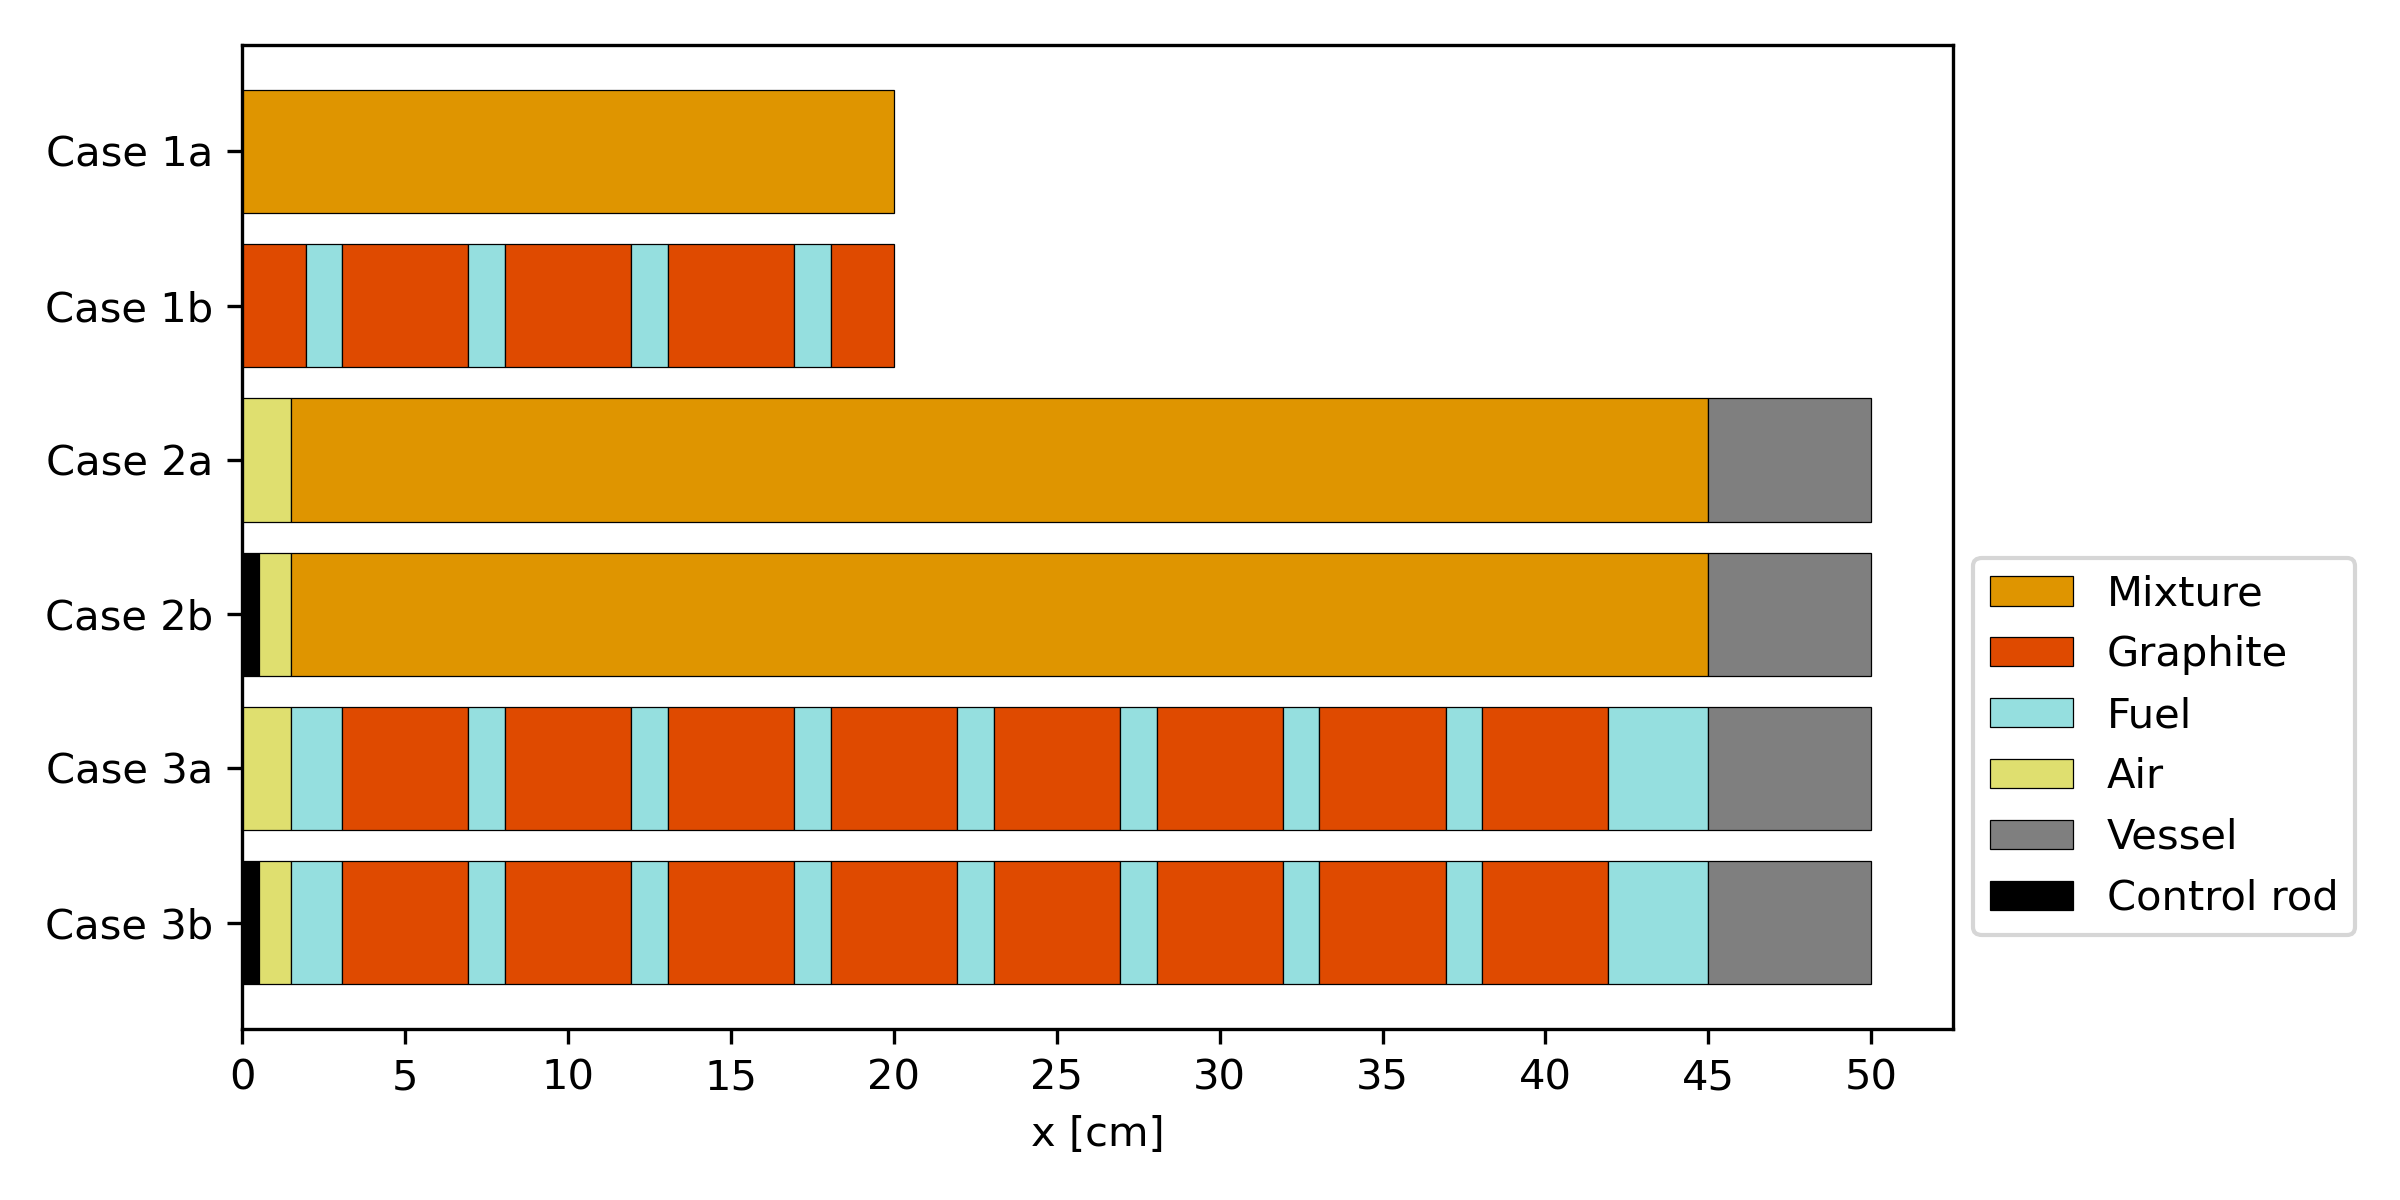
\includegraphics[width=0.8\columnwidth]{case-geometry}
  \caption{Geometries of the 1-D test cases. The material labeled ``mixture'' represents a
    homogeneous mixture of fuel and graphite at a ratio of 22.5\%-77.5\% by volume. All geometries
    have reflective boundary conditions on the boundary at $x=0$ cm. The right-side boundaries are
    reflective for Cases 1a and 1b, and vacuum for Cases 2a, 2b, 3a, and 3b.}
  \label{fig:case-geom}
\end{figure}

\section{Numerical Results \& Discussion}

Figure \ref{fig:1d-rho} shows the difference in reactivities of OpenMC-MG, $S_8$, neutron
diffusion, and hybrid methods relative to OpenMC-CE for all test cases. The standard deviations of
reactivity values from OpenMC-CE are approximately 40 pcm for Cases 1a and 1b and 60 pcm for the
rest as depicted by the blue highlighted area in Figure \ref{fig:1d-rho}. For Cases 1a and 1b, the
OpenMC-MG, $S_8$, and neutron diffusion methods show excellent agreement with OpenMC-CE as the
reactivity values fall within the one or two standard deviation range.
%
\begin{figure}[htb!]
  \centering
  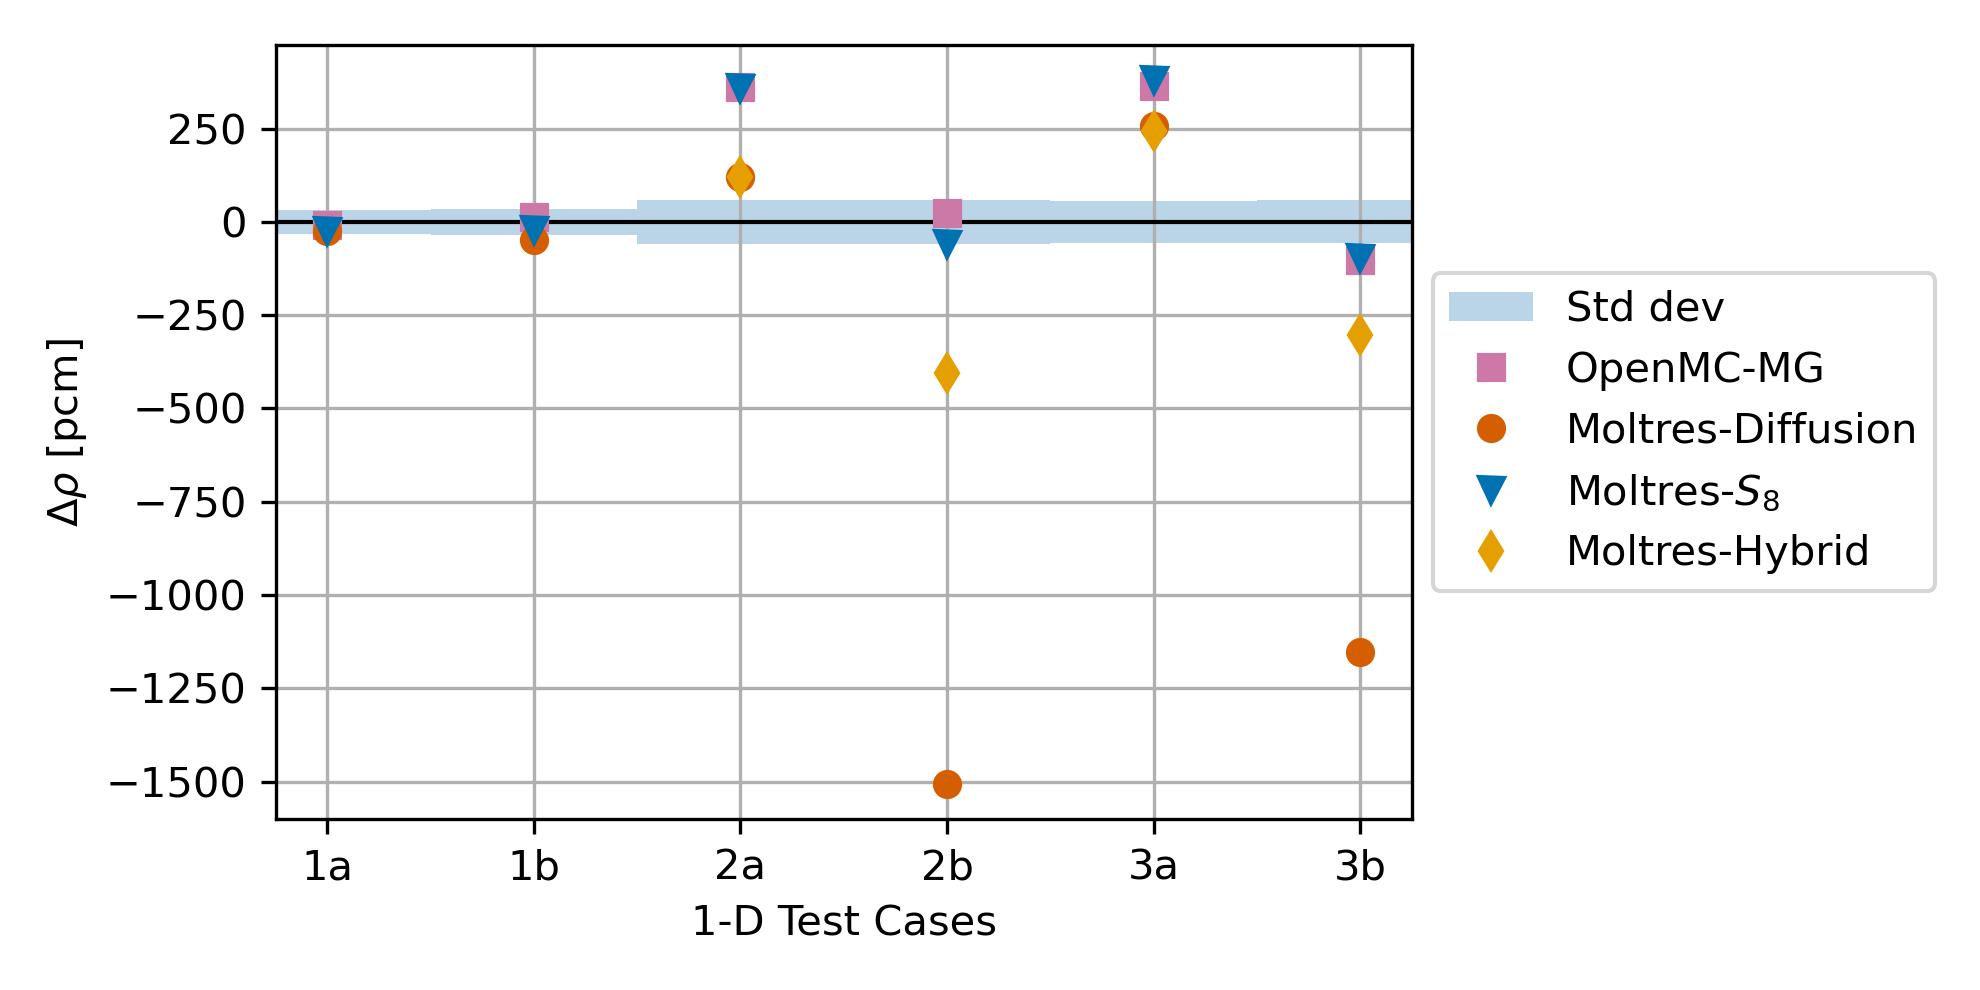
\includegraphics[width=0.8\columnwidth]{rho}
  \caption{Difference in reactivity $\rho$ of all neutronics methods investigated relative
  to OpenMC-CE.}
  \label{fig:1d-rho}
\end{figure}

For all cases, the OpenMC-MG and the $S_8$ methods show consistent agreement with one another. 
While they deviate from OpenMC-CE by approximately 350 pcm for Cases 2a and 3a, they fall within
two standard deviations of OpenMC-CE for Cases 2b and 3b. When increasing the maximum Legendre
polynomial order to approximate the angular dependence in $\Sigma_s^{g'\rightarrow g}$ from
2nd-order to 3rd-order, the reactivity changed by only 1 pcm. Therefore, we attribute the reactivity
discrepancies to the eight neutron energy group structure which remains the
only significant difference between OpenMC-CE and the multigroup methods.

The neutron diffusion and hybrid methods agree closely with one another for Cases 2a and 3a which
exclude the control rod region. This shows that the hybrid method provides similar $k_\text{eff}$
estimates to the neutron diffusion method in 1-D simulations without highly neutron-absorbing
regions. Compared to the OpenMC-MG and $S_8$ reactivity values, the neutron diffusion and hybrid
method reactivity values agree closer with the reference OpenMC-CE value. However, this is likely
due to favorable error cancellation.

In Cases 2b and 3b, the neutron diffusion method largely fails to accurately capture the
effect of introducing the control rod region as evidenced by the -1500 pcm and -1150 pcm
discrepancies relative to OpenMC-CE. The hybrid method fares better with -400 pcm and -300 pcm
discrepancies.

Moving the discussion to control rod worths, figure \ref{fig:1d-worth} shows the percentage
difference in rod worths for Cases 2 and 3 of OpenMC-MG, $S_8$, neutron diffusion, and hybrid
methods relative to OpenMC-CE. We calculated the rod worth estimates from each method by taking the
difference in reactivity between the ``rod out'' (a) and ``rod in'' (b) configurations of Cases 2
and 3. All neutronics methods overestimate the rod worth relative to OpenMC-CE, resulting in
positive percentage difference values observed in the figure.
The neutron diffusion methods clearly show up as outliers with rod worth estimates in excess
of 8\%. The remaining methods cluster around 2.5\% and 3\% percentage difference for Cases
2 and 3.

Given that the hybrid methods rely on transport corrections derived from the $S_N$ method, the
$S_8$ rod worth estimates serve as the
reference point for hybrid method verification. Additionally, errors arising from the multigroup
approximation affect both hybrid and $S_N$ simulations to similar degrees. The hybrid method
provides significant improvements in rod worth estimates over the neutron diffusion method.
%
\begin{figure}[htb!]
  \centering
  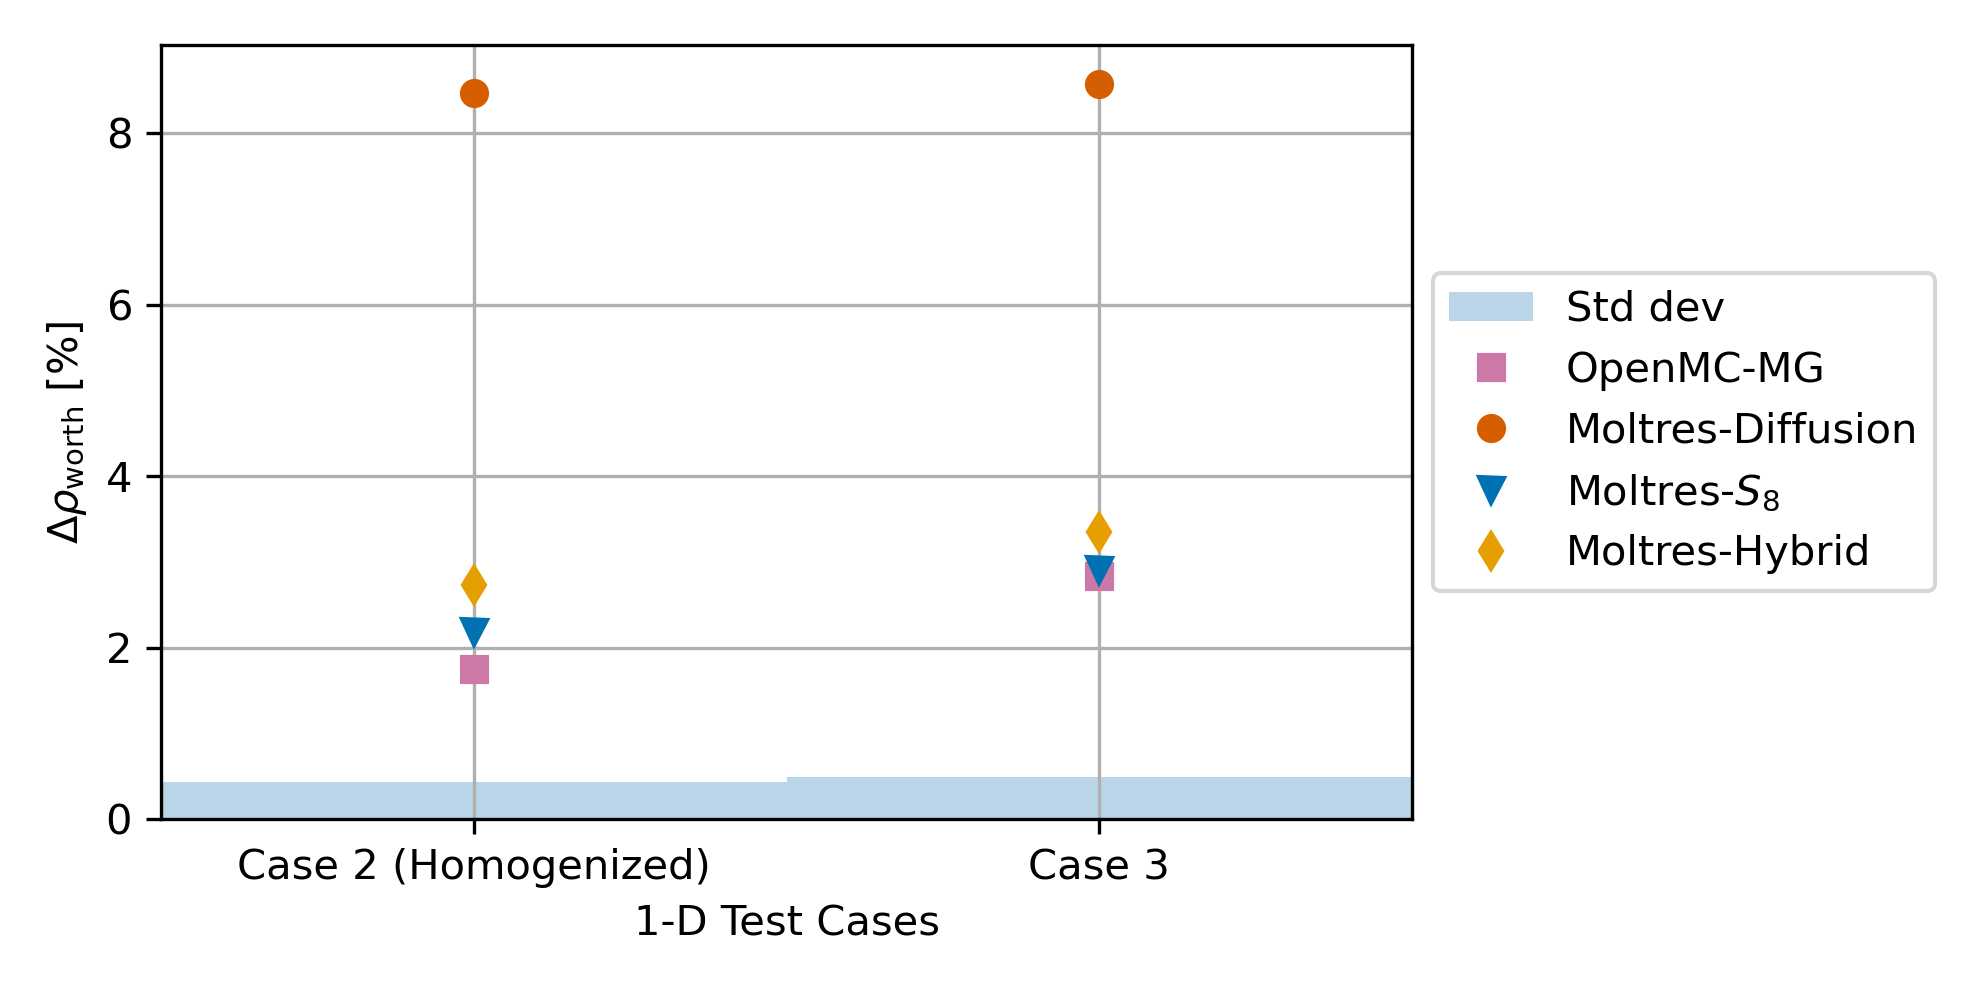
\includegraphics[width=0.8\columnwidth]{worth}
  \caption{Percentage difference in rod worth for Cases 2 and 3 of all neutronics methods
  investigated relative to OpenMC-CE.}
  \label{fig:1d-worth}
\end{figure}

Figure \ref{fig:3b-flux-diff} shows the absolute
difference in Case 3b neutron group flux distributions of the $S_8$, neutron diffusion, and
hybrid methods relative to OpenMC-MG, instead of OpenMC-CE, to eliminate discrepancies arising from
the multigroup approximation. Case 3b most closely resembles the actual \gls{MSRE} design with an
inserted rod.
The neutron diffusion and hybrid methods fare worse than the $S_8$ method at capturing the
oscillatory pattern in groups 1, 2, 5, 7, and 8 arising from the fuel-graphite lattice geometry
along $x=5$ cm to 10 cm. The neutron diffusion method
exhibits significant flux deviations in groups 1, 2, 7, and 8 near $x=0$ cm. The hybrid method
provides significant improvements in neutron flux distributions compared to the neutron diffusion
method as shown by the generally smaller flux difference values particularly near $x=0$ cm.

\begin{figure}[htb!]
  \centering
  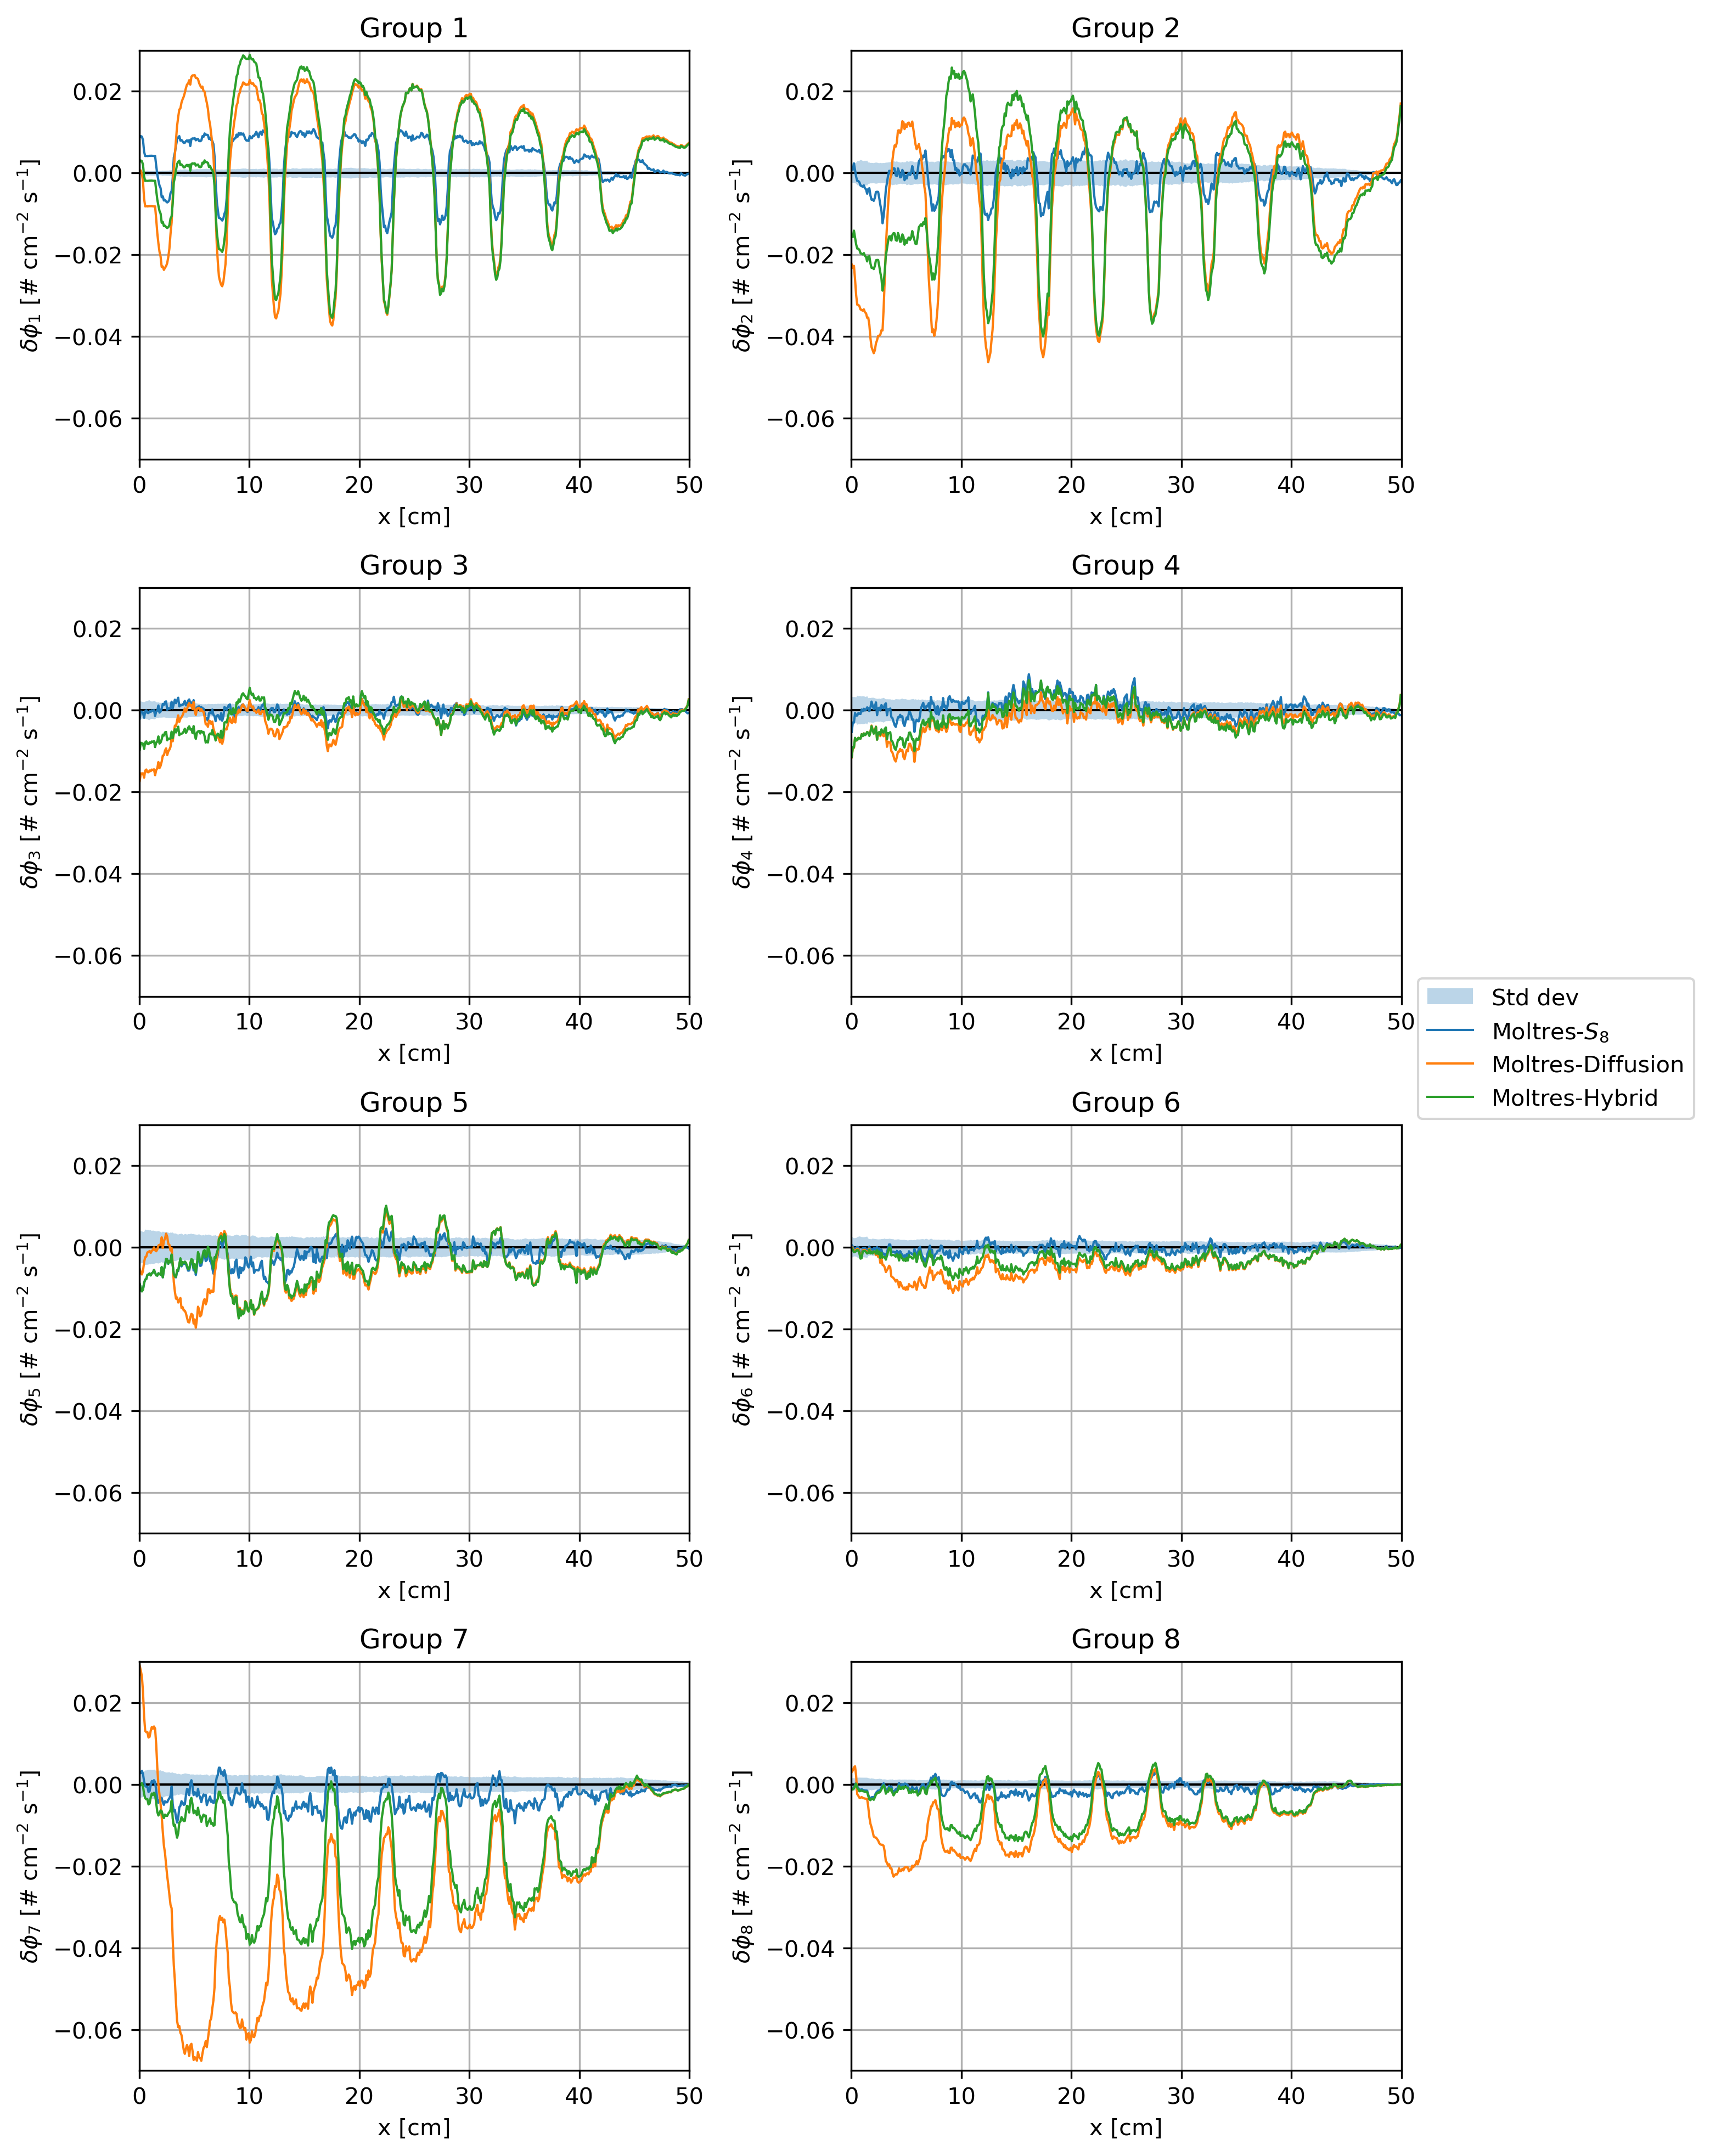
\includegraphics[width=\columnwidth]{case-3b-flux-diff}
  \caption{Absolute difference in neutron group flux distributions for Case 3b from $S_8$,
  neutron diffusion, and hybrid methods relative to OpenMC-MG.}
  \label{fig:3b-flux-diff}
\end{figure}

Figure \ref{fig:3b-drift} shows the drift correction parameter distribution in each neutron energy
group for Case 3b. We computed the reference drift distributions from reference flux
solutions of the standard $S_8$ method.
The drift correction parameters generated by the correction scheme match their respective reference
values within the correction subregion from $x=0$ cm to 10 cm except near the subregion boundary at
$x=10$ cm as previously discussed in Section \ref{sec:hybrid-algorithm}. The buffer region $V_1'$
completely encompasses the region near $x=10$ cm where the drift correction distributions deviate
from the reference distribution and are thus discarded.

\begin{figure}[htb!]
  \centering
  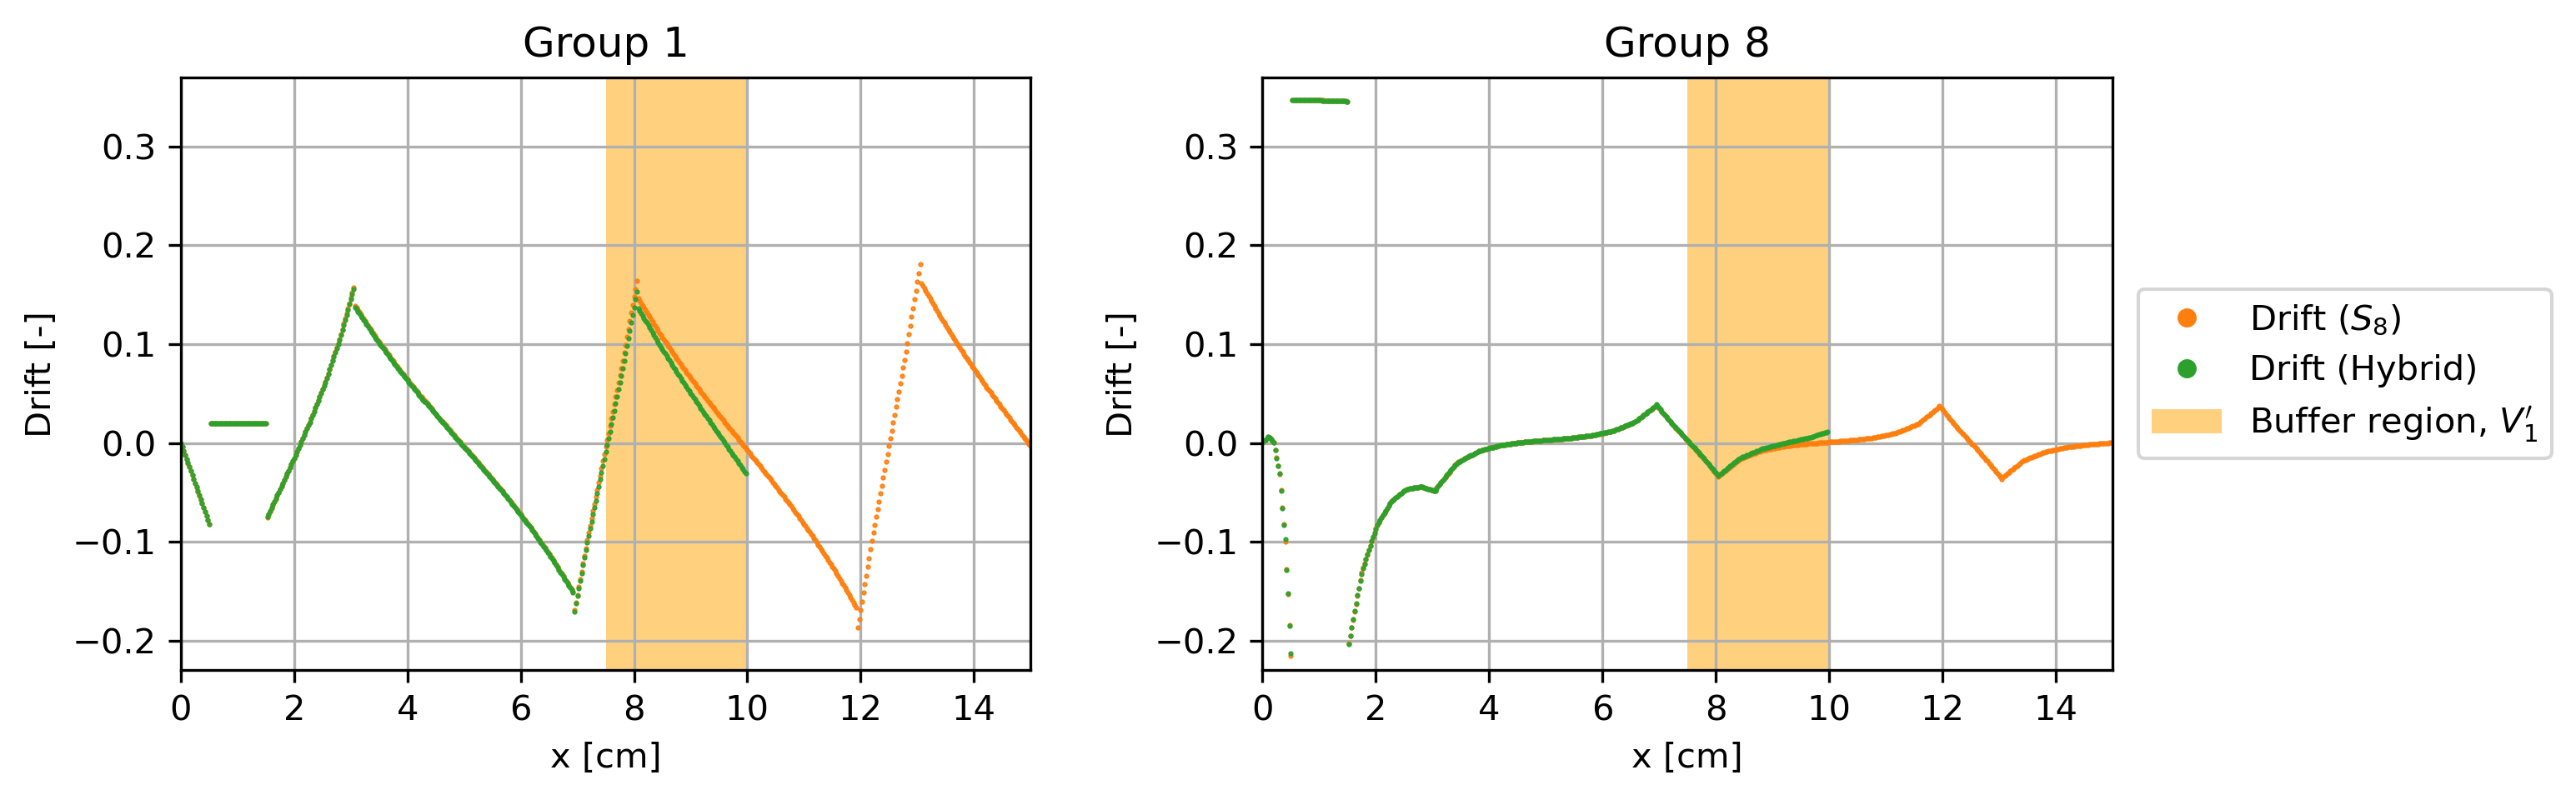
\includegraphics[width=\columnwidth]{case-3b-drift}
  \caption{Multigroup drift correction ($\vec{D}_g$) $x$-component distributions from the
  Moltres-hybrid and Moltres-$S_8$ solvers.}
  \label{fig:3b-drift}
\end{figure}

% The hybrid $S_N$-diffusion method relies on $S_N$ calculations in the correction subregion to
% generate flux corrections. Minimizing the size of the correction subregion and the $S_N$ subproblem
% is essential for the hybrid method to be computationally competitive for time-dependent full-core
% simulations. I investigated the effect of the correction subregion size on the $k_\text{eff}$ and
% control rod worth estimates with Cases 3a and 3b by varying the subregion sizes from 10 cm to 40 cm
% at 5 cm-intervals.
% 
% Figures \ref{fig:v1-size-a-k} and \ref{fig:v1-size-b-k} show the $k_\text{eff}$ estimates from the
% hybrid method for Cases 3a and 3b, respectively. In both cases, the $k_\text{eff}$ values initially
% decrease as the correction subregion sizes increase before reversing in trend when the subregion
% size reaches 35 cm and beyond. The $k_\text{eff}$ values vary by up to 164 pcm for Case 3a and 109
% pcm for Case 3b. An important observation here is that the $k_\text{eff}$ values do not
% monotonically converge towards the $k_\text{eff}$ estimate from the $S_8$ method. The data implies
% other significant sources of discrepancies exist beyond those being corrected in the
% correction subregion by the hybrid method.
% 
% \begin{figure}[htb!]
%   \centering
%   \includegraphics[width=\columnwidth]{correction-size-b-k}
%   \caption{$k_\text{eff}$ estimates from the hybrid method for Case 3b with different
%   correction subregion sizes. The horizontal lines indicate $k_\text{eff}$ estimates from the
%   OpenMC-CE, OpenMC-MG, and $S_8$ methods.}
%   \label{fig:v1-size-k}
% \end{figure}
% 
% Figure \ref{fig:v1-size-rho} shows the percentage difference in rod worth relative to OpenMC-CE. 
% Due to the identical trends observed in the $k_\text{eff}$ estimates of both cases, the control rod
% worth estimates do not change significantly when the correction subregion
% sizes change. This indicates limiting the correction subregion size to save
% computational cost on the expensive $S_N$ calculations has a negligible impact on rod worth
% estimates. The rod worth estimates for all investigated correction subregion sizes remain within
% 0.2\% of the $S_8$ method.
% 
% \begin{figure}[htb!]
%   \centering
%   \includegraphics[width=0.8\columnwidth]{correction-size-rho}
%   \caption{Percentage difference in rod worth from the hybrid method relative to OpenMC-CE for
%     Cases 3a and 3b with different correction subregion sizes. The horizontal lines indicate
%     equivalent rod worth differences from the OpenMC-MG and $S_8$ methods.}
%   \label{fig:v1-size-rho}
% \end{figure}

\section{CONCLUSIONS}

The reactivity and rod worth results show the hybrid method is able to accurately
reproduce rod worth estimates as long as the correction subregion size remains consistent. The
correction subregion size must also be sufficiently large to capture the highly neutron-absorptive
rod's influence on the neutron flux around the rod at $x=0$ cm. The drift correction parameter
distributions in Figure \ref{fig:3b-drift} indicate that the influence of the rod on the drift, and
consequently the flux, extend to approximately $x=5$ cm before the drift distribution settles on a
regular repeating pattern influenced by the fuel-graphite lattice structure. I applied a consistent
correction subregion size of 10 cm for Cases 2 and 3 since it sufficiently meets the requirements
discussed while also minimizing the computational cost of the $S_8$ subsolver. Other reactor
designs consisting of different material components may require different minimum correction
subregion sizes.

\section*{ACKNOWLEDGEMENTS}
Acknowledge the help of colleagues, and sources of funding, as appropriate.

\bibliographystyle{mc2025}
\bibliography{bibliography}

\end{document}
